\documentclass{article}

% --- Tight PDF output (no standalone.cls needed) ---
\usepackage[
  paperwidth=12cm,
  paperheight=5cm,
  margin=6mm
]{geometry}
\pagestyle{empty}

\usepackage{tikz}

\begin{document}
\begin{center}
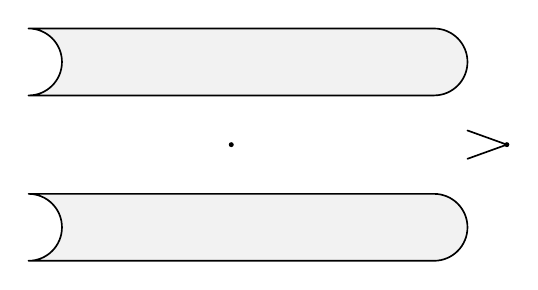
\begin{tikzpicture}[line cap=round, line join=round]

% ---------------- styles ----------------
\tikzset{
  hull/.style ={draw, line width=0.6pt, fill=gray!10},
  dot/.style  ={fill=black}
}

% ---------------- parameters ----------------
\def\L{6.0}      % pontoon length (without tip)
\def\W{0.85}     % pontoon width
\def\R{0.425}    % end radius (W/2 recommended)
\def\Gap{1.05}   % half spacing between pontoons
\def\Tip{0.50}   % forward marker length

% derived
\def\xLeft{-\L/2}
\def\xRight{\L/2}
\def\xcL{\xLeft+\R}
\def\xcR{\xRight-\R}
\def\yTop{\W/2}
\def\yBot{-\W/2}

% helper: draw one pontoon centered at y0 (single closed path)
\newcommand{\Pontoon}[1]{%
  \path[hull]
    (\xcL, #1+\yTop) -- (\xcR, #1+\yTop)
    arc[start angle=90, end angle=-90, radius=\R]
    -- (\xcL, #1+\yBot)
    arc[start angle=-90, end angle=90, radius=\R]
    -- cycle;
}

% ---------------- draw pontoons ----------------
\Pontoon{\Gap}
\Pontoon{-\Gap}

% ---------------- minimal forward marker (very subtle) ----------------
% a small open wedge at the bow to indicate direction (not filled, avoids clutter)
\draw[line width=0.6pt]
  (\xRight, 0.18) -- (\xRight+\Tip, 0) -- (\xRight, -0.18);

% ---------------- anchors ----------------
\coordinate (usvCenter) at (0,0);
\coordinate (usvBow)    at (\xRight+\Tip,0);
\coordinate (usvStern)  at (\xLeft,0);

\fill[dot] (usvCenter) circle (0.9pt);
\fill[dot] (usvBow)    circle (0.9pt);

\end{tikzpicture}
\end{center}
\end{document}